\documentclass{article}
\usepackage{amsmath}    % 수학 기호와 수식을 위한 패키지
\usepackage{graphicx}   % 이미지 삽입을 위한 패키지
\usepackage{hyperref}   % 하이퍼링크 사용을 위한 패키지
\usepackage{enumitem}   % 리스트 포맷 조정을 위한 패키지

\title{\textbf{Problem Set 1}}
\author{}
\date{}

\begin{document}

\maketitle

\section*{Problems}


\begin{enumerate}[label=\textbf{\arabic*.}]
    \item Identify the normalization condition that describes a wavefunction \( \Phi (x) \) expanded in terms of a complete orthonormal set of basis functions \( \{\phi_i (x)\} \) with coefficients \( \{c_i\} \).\\

    Since $\{\phi_i\}$ are a complete orthonormal set of basis, 
    $\Phi(x)$ can be expanded as $\sum_i c_i \phi_i(x)$ for some unique set of coefficients $\{c_i\}$. 
    Then, the normalization condition of $\Phi(x)$, $|\Phi(x)|^2 = 1$, can be written
    as $\int \left|\sum_i c_i \phi_i(x)\right|^2 dx = \int \sum_{i,j} c_i^* c_j 
    \phi_i^* \phi_j \, dx$.
    \begin{align*}
        1 &= \int |\Phi(x)|^2 \, dx \\
        &= \int \left| \sum_i c_i \phi_i(x) \right|^2 \, dx \\
        &= \int \left( \sum_i c_i \phi_i(x) \right) \left( \sum_j c_j^* \phi_j^*(x) \right) \, dx \\
        &= \int \left[ \sum_i \sum_j c_i c_j^* \phi_i(x) \phi_j^*(x) \right] \, dx \\
        &= \sum_i \sum_j c_i c_j^* \int \phi_i(x) \phi_j^*(x) \, dx \\
        &= \sum_i \sum_j c_i c_j^* \langle \phi_i | \phi_j \rangle \\
        &= \sum_i \sum_j c_i c_j^* \delta_{ij} \\
        &= \sum_i c_i c_i^* \\
        &= \sum_i |c_i|^2
    \end{align*}

    \item Consider the wavefunction
    \[
    \Psi (x) = 0.6i\phi_1 (x) + 0.1\phi_2 (x) + c_3\phi_3 (x) - 0.5\phi_4 (x),
    \]
    where \( \Psi (x) \) is normalized, \( \hat{O}\phi_j (x) = j\phi_j (x) \), and \( \{\phi_j (x)\} \) form an orthonormal set.
    \begin{enumerate}[label=\textbf{(\alph*)}]
        \item Calculate the magnitude of \( c_3 \).
        \begin{align*}
            1       &= 0.6i \cdot (-0.6i) + 0.1^2 + |c_3|^2 + 0.5^2 \\
                    &= 0.36 + 0.01 + |c_3|^2 + 0.25 \\
                    &= 0.62 + |c_3|^2 \\
            |c_3|^2 &= 0.38 \\
            c_3 &= \sqrt{0.38} \\
        \end{align*}
        \item Plot the expected distribution of the outcomes of repeated measurements of the operator \( \hat{O} \).
        \begin{figure}
            \centering
            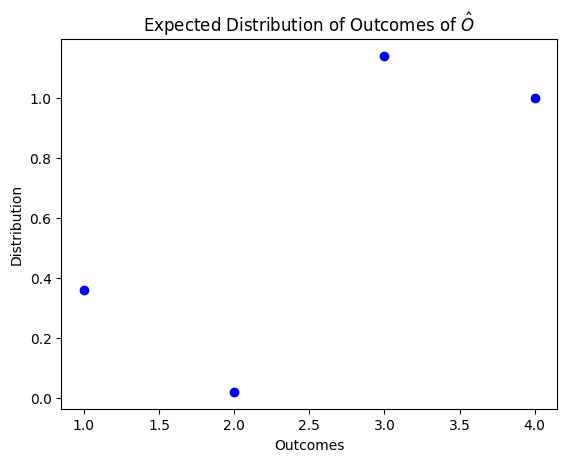
\includegraphics[width=0.5\linewidth]{2-b answer.png}
            \caption{Plot of the probability of getting the eigenvalue $j_i$ in a measurement of the property $O$}
            \label{fig:enter-label}
        \end{figure}
        
        \item Compute \( \langle \hat{O} \rangle \).
        \begin{flalign*}
            &\int \Psi^*(x) \, \hat{O} \, \Psi(x) \, dx \\
            &= \int \Psi^*(x) \, \hat{O} \left( 0.6i \phi_1(x) + 0.1 \phi_2(x) + c_3 \phi_3(x) - 0.5 \phi_4(x) \right) \, dx \\
            &= \int \Psi^*(x) \left( 0.6i \hat{O} \phi_1(x) + 0.2 \hat{O} \phi_2(x) + 3c_3 \hat{O} \phi_3(x) - 2\hat{O} \phi_4(x) \right) \, dx \\
            &= \int \left( 0.6i \phi_1(x) + 0.1 \phi_2(x) + c_3 \phi_3(x) - 0.5 \phi_4(x) \right)^* \\
            &~~~~\left( 0.6i \hat{O} \phi_1(x) + 0.2 \hat{O} \phi_2(x) + 3c_3 \hat{O} \phi_3(x) - 2 \hat{O} \phi_4(x) \right) \, dx. \\
            &= \int \left( 0.6i \phi_1(x) + 0.1 \phi_2(x) + c_3 \phi_3(x) - 0.5 \phi_4(x) \right)^* \\
            &~~~~\left( 0.6i\cdot 1 \phi_1(x) + 0.2\cdot \phi_2(x) + 3c_3 \cdot \phi_3(x) - 2 \cdot 4 \phi_4(x) \right) \, dx. \\
            &= 0.36 + 0.02 + 3|c_3|^2 + 1 ~~ \text{(used normalization condition of basis)}\\
            &= 0.36 + 0.02 + 1.14 + 1 \\
            &= 2.52 &&
        \end{flalign*}
    \end{enumerate}

    \item Prove that Hermitian operators only have real eigenvalues.
    \begin{align*}
        \hat{H}^\dagger &= \hat{H} \\
        \hat{H} \Psi &= \alpha \Psi \\
        \int \Psi^* \, \hat{H} \, \Psi \, dx &= \alpha \int |\Psi|^2 \, dx \\
        \text{Complex conjugate of the above:} \\
        \int \Psi \, \hat{H}^\dagger \, \Psi^* \, dx &= \alpha^* \int |\Psi|^2 \, dx \\
        \int \Psi^* \, \hat{H} \, \Psi \, dx &= \alpha^* \int |\Psi|^2 \, dx \\
        \alpha &= \alpha^* ~~ (\text{since}~\Psi \neq 0)
    \end{align*}

    \item Complete the Python exercise in \texttt{problemset1.ipynb}.
    \begin{enumerate}[label=\textbf{(\alph*)}]
        \item Download and install Python and Jupyter Notebook.
        \item Run the Jupyter notebook \texttt{problemset1.ipynb} using \texttt{shift-enter} to run each cell.
        \begin{enumerate}[label=\textbf{\roman*.}]
            \item Method 1: Run \texttt{Anaconda Navigator}, open \texttt{JupyterLab}, and import the notebook with the \texttt{Upload file} icon (icon with an up arrow).
            \item Method 2: Navigate to the folder on your computer that contains \texttt{problemset1.ipynb}, open the command line (terminal), and type \texttt{jupyter notebook problemset1.ipynb}.
        \end{enumerate}
        \item To gain a greater understanding of the type of Python code used in class, test how the output of the program varies as you change variables, function names, etc.
        \item Complete and submit the answer to the problem marked “Problem Set Exercise” at the end of \texttt{problemset1.ipynb} alongside this problem set. Be careful to always label axes.
    \end{enumerate}
\end{enumerate}

\end{document}